\documentclass[12pt]{article}

% Language setting
% Replace `english' with e.g. `spanish' to change the document language
\usepackage[spanish]{babel}

% Set page size and margins
% Replace `letterpaper' with `a4paper' for UK/EU standard size
\usepackage[letterpaper,top=2cm,bottom=2cm,left=3cm,right=3cm,marginparwidth=1.75cm]{geometry}

% Useful packages
\usepackage{amsmath}
\usepackage{graphicx}
\usepackage[colorlinks=true, allcolors=blue]{hyperref}
\usepackage{authblk}
\usepackage[font=large,labelfont=bf]{caption}
\usepackage{float}
\usepackage{tikz}
\usepackage{amsfonts}
\usepackage{amsthm}
\usepackage{amsmath}
\usepackage{amssymb}
\usepackage{listings}
\usepackage{xcolor}
\usepackage{booktabs}
\usepackage{siunitx}
\usepackage{array}
\usepackage{dcolumn}
\usepackage{bbm}
\usepackage{subfig}
\usepackage{scrextend}
\usepackage{hyperref}



\addto\captionsspanish{
\def\listtablename{\'Indice de tablas}%
\def\tablename{Tabla}}
\deffootnote[2em]{2em}{1em}{\textsuperscript{\thefootnotemark}\,}


\title{\textbf{Taller 1 Big Data \& Machine learning}}
\author{Hugo Sabogal, Gabriela Pérez, Maria Paula Osuna, Juan Andrés Silva}
\affil{Universidad de los Andes \\ Facultad de Economía}

\date{\today }



\begin{document}
\maketitle

\begin{center}
    \href{https://github.com/Hugo-Andres-Sabogal-Perez/Problem-set-1}{\label{repo}Repositorio de GitHub}
\end{center}


\section{Introducción}

La evasión de impuestos representa un problema significativo para la economía colombiana, ya que puede incidir negativamente en el desarrollo del país y en las finanzas nacionales. En este contexto, se busca focalizar la atención en el impuesto a la renta pagado por las personas naturales, siendo este tributo principalmente abonado por ciudadanos mayores de 18 años y empleados. La situación de este impuesto, calculado según los ingresos de los ciudadanos, no presenta un panorama favorable en Colombia, como lo evidencia la información de la DIAN que señala que, en 2021, las personas naturales evadieron alrededor de 42 billones de pesos, equivalente al 3.6\% del PIB de ese año (DIAN, 2021). \\


Dada la alarmante situación descrita anteriormente se quiere mencionar la importancia de detectar la evasión de impuestos para preservar la integridad del sistema fiscal colombiano. La recaudación tributaria desempeña un papel vital en la financiación de servicios públicos esenciales, tales como infraestructura, salud, seguridad y educación. Por otro lado, la evasión fiscal genera desequilibrios en la distribución de la carga impositiva. Identificar a personas mayores de 18 años, especialmente empleadas, que eluden sus obligaciones tributarias, puede contribuir a la estabilidad de un sistema tributario eficiente, fomentando el cumplimiento de las obligaciones fiscales y fortaleciendo la confianza en las instituciones gubernamentales. Además, combatir la evasión fiscal puede tener un impacto significativo en el desarrollo del país al mejorar la situación del déficit fiscal y permitir una distribución más equitativa de los recursos. \\


Con el propósito de abordar la problemática mencionada anteriormente, es relevante destacar el surgimiento de modelos de predicción de ingresos como herramientas fundamentales tanto para el cálculo de impuestos como para la detección de posibles casos de fraude, permitiendo identificar a aquellos individuos que potencialmente evaden sus obligaciones fiscales. Este documento se enfoca en la identificación de posibles evasores de impuestos mediante el uso de modelos predictivos como herramienta clave en este proceso. \\

El presente trabajo contribuye a la literatura de economía laboral dado que en él se encontraron resultados que favorecen ésta. En primer lugar, se encontró que la edad es un factor que tiene efecto positivo sobre el logaritmo del salario pero tiene rendimientos marginales decrecientes y es aproximadamente cuando las personas alcanzan los 50 años es en promedio llegan al mayor salario alcanzado. En segundo lugar, se encontró evidencia de la existencia de una brecha salarial condicionada entre hombres y mujeres la cual en 2014 era de en promedio 4.5\%. Por último, se testearon estos dos modelos conjunto 5 adicionales. A partir de esto se llegó a la conclusión que los métodos de selección de backwards y forward eligen modelos que se desempeñan mejor en términos predictivos que los modelos utilizados por la literatura económica. \\


\section{Datos}

\subsection{Descripción}

Los datos utilizados a lo largo del presente trabajo provienen de la Gran Encuesta Integral de Hogares (GEIH), la cual se realiza para capturar información sobre las condiciones de empleo de las personas y demás características generales de la población a nivel nacional, regional, departamental y para cada una de las capitales departamentales\footnote{Esta Información fue recuperada de la página oficial del Departamento Administrativo Nacional de Estadística.} . Específicamente, se utilizaron datos del reporte de “Medición de Pobreza Monetaria y Desigualdad” para Bogotá durante el año 2018. Además de contener las variables especificadas por el reporte, la base de datos utilizada contiene variables adicionales que fueron ya dadas para la realización del trabajo.

\subsection{Procesamiento de datos}

En la página web para acceder a los datos, éstos se encontraban divididos en 10 partes llamadas “Data Chunk \#\footnote{El símbolo # se reemplaza de 1 a 10 dependiendo del número de parte al que se hace referencia.} ” con un total de 32.177 observaciones. Para poder tener acceso a una única base de datos que contuviese la totalidad de las observaciones fue necesario realizar el proceso de “web scraping\footnote{Este proceso se encuentra desde la línea 3 hasta la línea 40 del R Script.}”. En primer momento, se realizó una función en la que se importó el link de la página web que contenía las 10 partes de la base de datos, dentro de esta misma función llamamos los datos contenidos en “Data Chunk 1” y los agrupamos en una nueva base llamada “datos”, estos datos fueron encadenados a partir de las variables de texto (strings). En segundo momento, aún dentro de la función, se creó un loop que permitiera añadir las filas que existieran desde “Data Chunk 2” hasta “Data Chunk 10” en la base “datos”; es importante recalcar que estos dos procesos contenidos dentro de la función fueron llamados a partir de su HTML.

\subsection{Limpieza de datos}

Después del procesamiento de los datos y ya teniendo acceso a la base de datos conjunta se procedió a realizar una limpieza de esta para eliminar cualquier tipo inconsistencia que ponga en riesgo la confiabilidad y calidad de los resultados. En primer lugar, se filtraron los datos que se utilizarán según las instrucciones dadas, personas con 18 años o más y quienes están empleados\footnote{Para esto se escogió la variable ocu, la cual toma el valor de 1 si la persona pertenece a la población ocupada, es decir quienes tienen un empleo formal o ejercen una actividad independiente y han trabajado al menos una hora en la semana de referencia.}. Continuando con esto, se crea, aparte, una nueva base en la que se incorporan los nombres de las estadísticas descriptivas que son más relevantes mostrar (el nombre de la variable, los misssing values, su media y su desviación estándar). Dado que esta información se encuentra vacía, se procede a realizar el conteo de los missings y el cálculo de la media y la desviación estándar para cada una de las variables dentro de la base; una vez llenada esta información, se tiene ahora una nueva base llamada “ED”.  \\

A partir de ésta, se filtran dichas variables que son constantes (es decir que tienen una desviación estándar igual a cero) y se eliminan, se observa además que dentro de la variable de interés (Salario medido en horas) hay un alto número de missing values (aproximadamente 6.000), por lo que antes de ser eliminadas, se analizó si éstos podían ser recuperados utilizando la variable de ingresos totales medidos en horas menos los ingresos no laborales medidos en horas. Sin embargo, se encontró que en éstas había un mayor número de missings (11.000 aproximadamente), por lo que se concluyó que lo mejor era deshacerse de dichas observaciones y se procedió a eliminarlas de la base de datos.\\

Después de esto, conjunto a un análisis estadístico y con la ayuda del diccionario con el que se contaba sobre las variables, se decidió crear una nueva base de datos con el nombre “base” que contuviese la variable dependiente, las variables explicativas que se utilizarían durante el trabajo y los controles necesarios para evitar un sesgo por variable omitida o cualquier problema que indujera endogeneidad en los modelos a realizar.

\subsection{Estadísticas descriptivas}

La base de datos anteriormente mencionada contiene 11 variables las cuales se explican a continuación:

\begin{enumerate}
    \item [\textbf{1.}] \textbf{age:} corresponde a la edad que tiene una persona medida en años, esta es fundamental para el desarrollo de los modelos por dos razones: primero, será la variable explicativa del primer modelo y segundo, actuará como control en el segundo modelo.
    \item [\textbf{2.}] \textbf{oficio:} corresponde a una variable categórica que va de 1 hasta 99, en cada uno de estos números se clasifican profesiones, así, el valor que tome cada observación indica la profesión de esta. Será utilizada como un control, pues bien, el salario de una persona depende de su profesión.
    \item [\textbf{3.}] \textbf{formal:} es una variable dummy que toma el valor de 1 si la persona hace parte de la población formal, ésta es importante tenerla entre los controles dado que la literatura colombiana ha expuesto que las personas pertenecientes al sector formal reciben mejor salario y/o beneficios laborales.
    \item [\textbf{4.}] \textbf{maxEducLevel:} es una variable categórica que toma valores entre 1 y 9 dependiendo del nivel de educación máximo que recibió una persona. Esta se utilizará como control dado que se relaciona positivamente con el salario de una persona.
    \item [\textbf{5.}] \textbf{Orden:} es la llave de la persona, es decir un número que identifica a cada individuo de la base.
    \item [\textbf{6.}] 6.	\textbf{P7040:} es una variable binaria que informa si la persona además de su ocupación principal tiene otro trabajo. Esta es importante tomarla como variable de control dado que al tener 2 o más trabajos puede sugerir que se tienen mayores ingresos salariales.
    \item [\textbf{7.}] \textbf{sex:} esta variable corresponde a una dummy que toma el valor de 1 si la persona es hombre y 0 si es mujer. Esta es importante dado que a partir de esta se realiza una transformación para obtener una dummy que tome el valor de 1 si la persona es mujer y 0 de lo contrario, teniendo así otra de las variables explicativas que se utilizarán en el desarrollo del trabajo.
    \item [\textbf{8.}] \textbf{sizeFirm:} esta variable define el número de trabajadores de la firma en la que una persona trabaja. Como es bien sabido, las personas en multinacionales o grandes empresas suelen reportar mayores salarios que aquellas que trabajan en pequeñas y medianas empresas. Por esto, es fundamental agregarla como control en el trabajo..
    \item [\textbf{9.}]\textbf{y\_ing\_lab y ln\_sal:}la primera corresponde al salario de una persona medido en horas en términos monetarios, la segunda es el logaritmo de éste. Estas corresponden a las variables de interés. 

    
    \item [\textbf{10.}] \textbf{HoursWorkUsual:} esta variable es el último control que se utilizará dentro del trabajo y corresponde al número de horas trabajas semanalmente. Es importante dado que éstas definen el salario que gana cada persona (entre más horas trabaja una persona, mayor será el salario que recibe ésta).
    
\end{enumerate}

A partir de esto se realizaron una serie de gráficas y una tabla que resume las estadísticas descriptivas más importantes para cada una de ellas: el número de observaciones, su media, su desviación estándar, su valor mínimo y su valor máximo. Estas se muestran a continuación:

\begin{figure}[htbp]
  \caption{Distribución de salario}\label{fig:hists}
  \hspace{-2cm}
  \subfloat[Salario en logaritmo\label{subfiga:hist}]{
    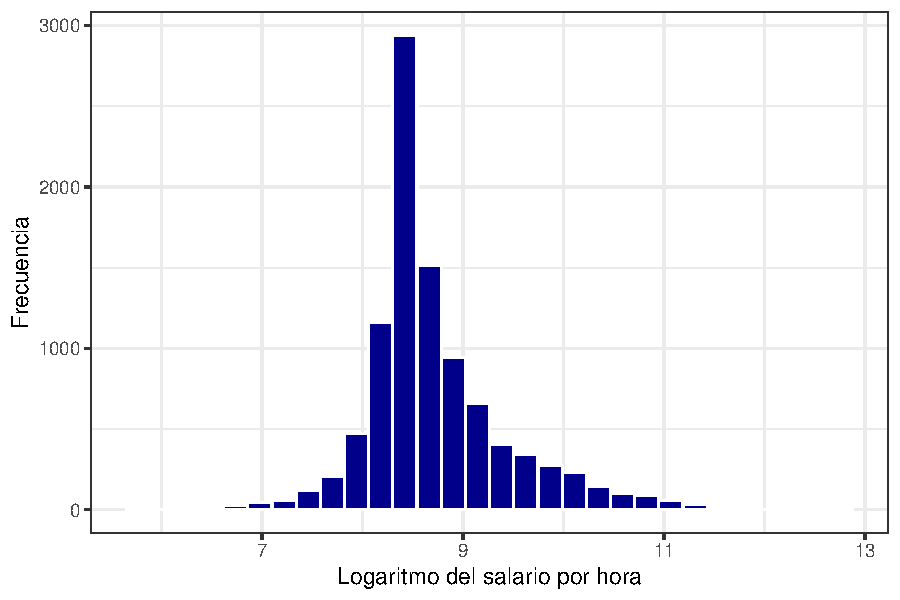
\includegraphics[width=0.6\textwidth, align=l]{imagenes/histograma.pdf}}
  \subfloat[Salario en niveles\label{subfigb:hist}]{
    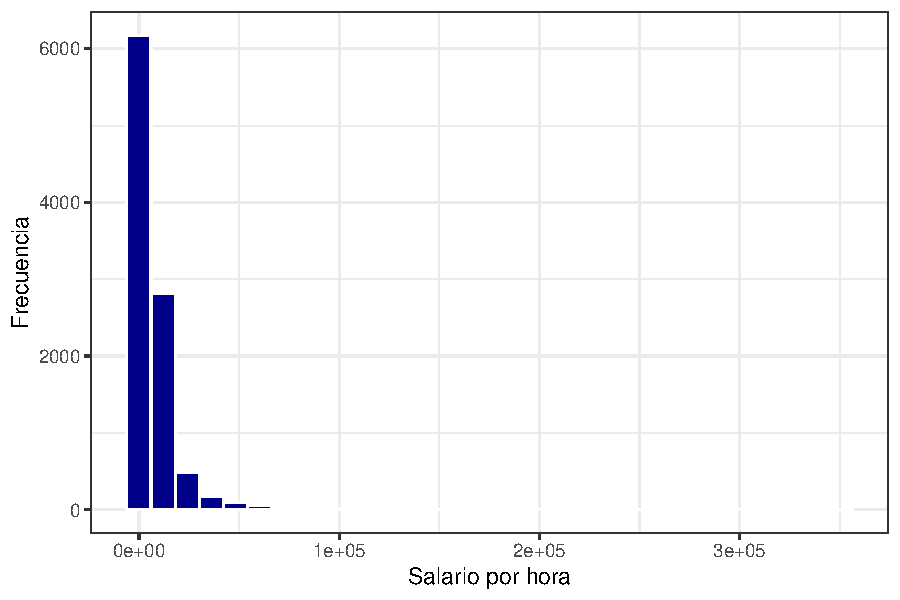
\includegraphics[width=0.6\textwidth, align=l]{imagenes/histograma_sal.pdf}}
    \begin{center}
        \footnotesize{\textbf{Fuente:} Elaboración propia con GEIH, 2024.}
    \end{center}
\end{figure}





En primer lugar, observando tanto la Figura \ref{subfiga:hist} como la Gráfica \ref{subfigb:hist}, se evidencia que transformar el salario por hora utilizando su logaritmo es necesario para corregir la asimetría que se observa en la distribución de los datos especialmente si existen muchas observaciones concentradas en niveles bajos de salario (tal como se evidencia en la primera gráfica). Además, esto permite una interpretación más sencilla de los coeficientes como cambios porcentuales en lugar de absolutos. Por último, esta transformación estabiliza la varianza de los errores de esta variable. Así, evidenciamos que el logaritmo del salario por hora se acerca a una distribución normal. \\

Ahora bien, teniendo en cuenta la definición inicialmente proveída, se muestra la tabla de estadísticas descriptivas de las variables:

\begin{table}[H] \centering 
  \caption{Estadísticas Descriptivas} 
  \label{} 
\begin{tabular}{@{\extracolsep{5pt}}lccccc} 
\\[-1.8ex]\hline 
\hline \\[-1.8ex] 
Variable & \multicolumn{1}{c}{N} & \multicolumn{1}{c}{Media} & \multicolumn{1}{c}{Dev. Est.} & \multicolumn{1}{c}{Min} & \multicolumn{1}{c}{Max} \\ 
\hline \\[-1.8ex] 
Edad & 9,889 & 36.227 & 12.006 & 18 & 86 \\ 
Oficio & 9,889 & 48.322 & 27.430 & 1 & 99 \\ 
Formal & 9,889 & 0.767 & 0.422 & 0 & 1 \\ 
Nivel educativo & 9,888 & 6.098 & 1.106 & 1 & 7 \\ 
Segundo trabajo [1=si] & 9,889 & 0.031 & 0.174 & 0 & 1 \\ 
Sexo[1=Hombre] & 9,889 & 0.503 & 0.500 & 0 & 1 \\ 
Tamaño firma & 9,889 & 3.921 & 1.333 & 1 & 5 \\ Salario & 9,889 & 8,796.308 & 12,790.120 & 326.667 & 350,583.300 \\ 
Horas trabajadas & 9,889 & 48.025 & 12.151 & 1 & 130 \\ 
ln(Salario) & 9,889 & 8.724 & 0.726 & 5.789 & 12.767 \\ 
\hline 
\hline\end{tabular} 
\begin{center}
    \footnotesize{\textbf{Fuente:} Elaboración propia con GEIH, 2024.}
\end{center}
\end{table} 



A partir de ésta se pueden resaltar principalmente que puede que existan datos atípicos en la variable de interés, el salario por hora, pues vemos que su valor máximo es de 350.583 COP y su media es de 8.796 COP, esto sugiere, inicialmente, que es necesario analizar a mayor profundidad los valores de esta variable para evitar tener relaciones equívocas que resulten en una mala estimación. Adicionalmente, al momento de realizar las estimaciones es necesario que tanto las variables categóricas como binarias se vuelvan más bien dummies\footnote{Para esto dentro de las estimaciones en estas variables se utilizó el comando format().}. 

        \begin{figure}[H]
            \caption{Logaritmo del salario vs edad}
            \centering
            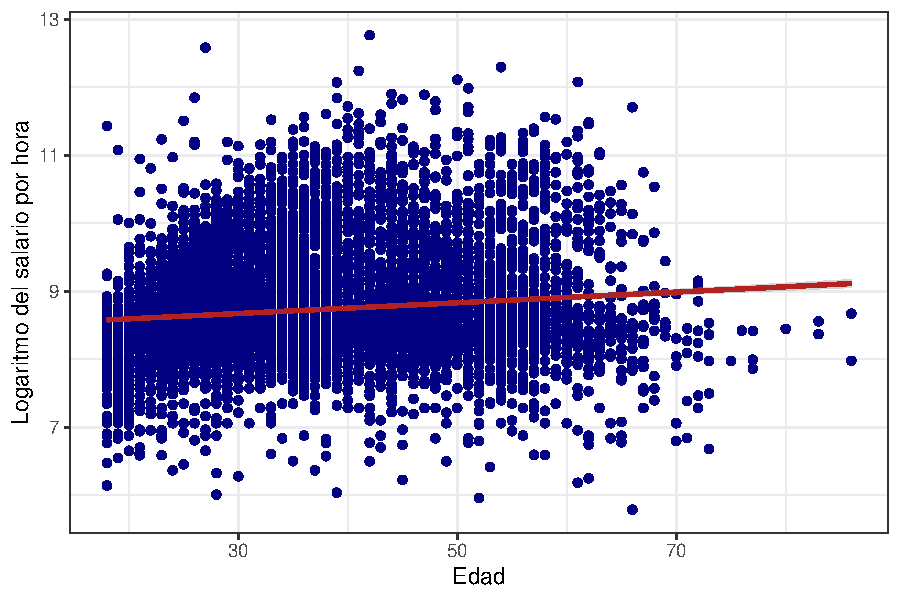
\includegraphics[width=0.7\textwidth]{imagenes/dispersion.pdf}
             \label{fig:scatter1}
            \begin{minipage}{7\textwidth}
            \footnotesize
            \hspace{3cm} Fuente: Elaboración propia con GEIH 2024.
       
            \end{minipage}
        \end{figure}
        \begin{figure}[H]
            \caption{Salario promedio por edad}
            \centering
            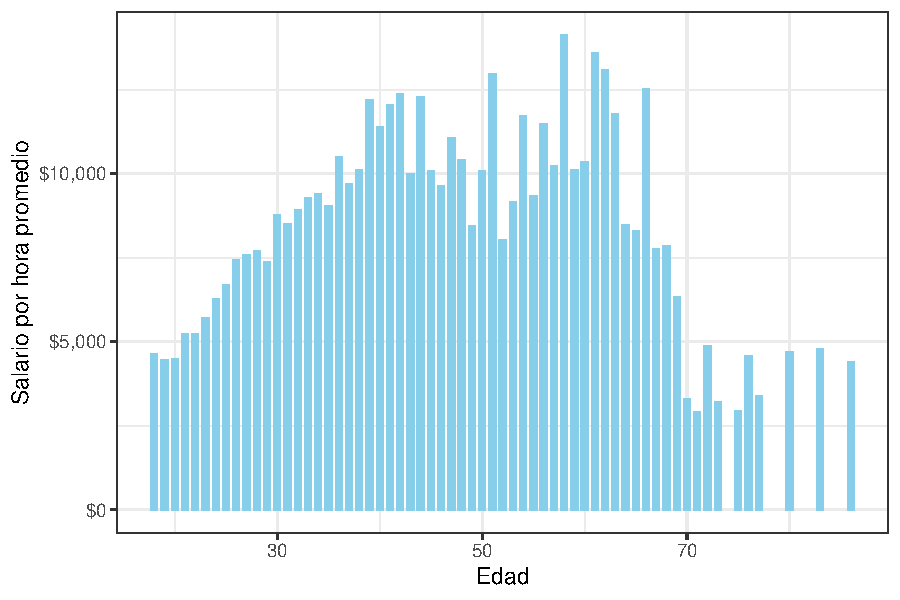
\includegraphics[width=0.7\textwidth]{imagenes/barras2.pdf}
             \label{fig:barras_sal}
            \begin{minipage}{7\textwidth}
            \footnotesize
            \hspace{4cm} Fuente: Elaboración propia con GEIH 2024.
       
            \end{minipage}
        \end{figure}
        \begin{figure}[H]
            \caption{Salario promedio por sexo}
            \centering
            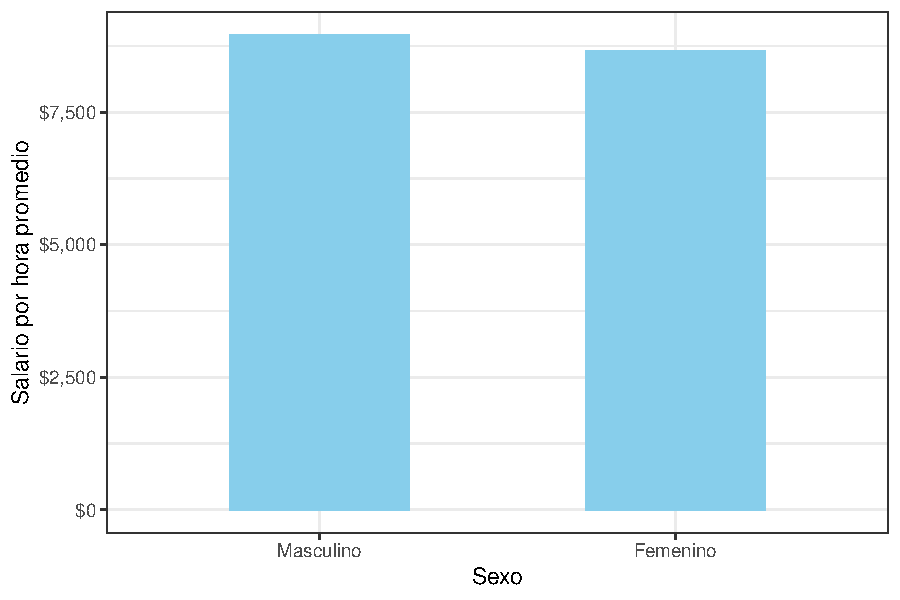
\includegraphics[width=0.7\textwidth]{imagenes/barras1.pdf}
             \label{fig:barras_sex}
            \begin{minipage}{7\textwidth}
            \footnotesize
            \hspace{4cm} Fuente: Elaboración propia con GEIH 2024.
       
            \end{minipage}
        \end{figure}


Continuando con esto, es necesario en principio observar las posibles relaciones que arrojarán las estimaciones de manera gráfica. Por esto, se crearon las gráficas \ref{fig:scatter1},\ref{fig:barras_sal} y \ref{fig:barras_sex}. A partir de la gráfica \ref{fig:scatter1} se observa que existe una relación positiva entre la edad en años y el logaritmo del salario por hora. Observando la gráfica \ref{fig:barras_sal} esta relación se confirma cuando observamos que a medida que aumenta la edad, el salario promedio de las personas aumenta. Sin embargo, de esta es importante recalcar que llegada cierta edad, el salario promedio empieza a disminuir nuevamente. Esto se debe a lo que la literatura llama los retornos negativos de la edad sobre el salario, esto quiere decir que solo hasta una edad es que la relación positiva entre estas variables se mantiene, después se vuelve negativa. Por último, a partir de la gráfica \ref{fig:barras_sex} se puede evidenciar que el salario promedio para los hombres es mayor (no por mucho) que el de las mujeres, esto se explica por la persistencia de una desigualdad de género en Colombia.

\section{Análisis de inferencia}

\subsection{Perfil edad salario}

Inicialmente se corrió un modelo del logaritmo del salario por hora contra la edad y la edad al cuadrado. A continuación, se muestra la tabla de resultados sobre esta estimación:

\input{tablas/reg1 }
Es importante recalcar que la interpretación de estos coeficientes no puede ser directa dado que los efectos de la edad sobre el salario no son constantes, esto ocurre dado que la edad tiene rendimientos marginales decrecientes sobre el salario. Ahora bien, es necesario para su interpretación que se realice el cálculo del efecto marginal que se encuentra a continuación, posteriormente, éste debe evaluarse en el promedio de la variable.

$$\frac{\partial ln(w)}{\partial age}=\beta_2+2 \beta_3\age$$

Reemplazando los coeficientes de resultados y el promedio de la variable edad en la ecuación tenemos, obtenemos que:


$$\frac{\partial ln(w)}{\partial age}=0.07032+2 (-0.000784)(36.227)=0.0135$$

Ya teniendo este resultado se puede concluir que a ante un aumento de un año de una persona, en promedio el salario aumenta en promedio 1.35\% teniendo en cuenta que este aumento es marginalmente decreciente (si se realiza la segunda derivada se espera que sea negativo este efecto). Tal como se observa en la tabla, estos resultados son estadísticamente significativos al 1\%, esto quiere decir que la edad de una persona es una buena variable para explicar la variación del logaritmo del salario por hora. Sin embargo, cuando se observa el $R^{2}$ y $R^{2}$ ajustado se evidencia que este modelo no explica en su mayoría la variación de la edad sobre el salario, de hecho, solo explica el $4\%$ aproximadamente. Adicionalmente, al no estar controlando por ningún otro efecto diferente al de la variable explicativa sobre la de interés se observa que el $R^2$ ajustado es el mismo que el $4\%$ descrito anteriormente, esto significa entonces que el modelo no cuenta con ningún ajuste que le de algún valor predictivo.
\\

Ahora bien, para analizar a mayor profundidad los rendimientos decrecientes de la edad sobre el salario se realizó un gráfico de dispersión en el que aparece el perfil estimado de edad-ganancias implícito en el modelo previamente analizado y su respectivo intervalo de confianza:

        \begin{figure}[H]
            \caption{Logaritmo del salario vs edad}
            \centering
            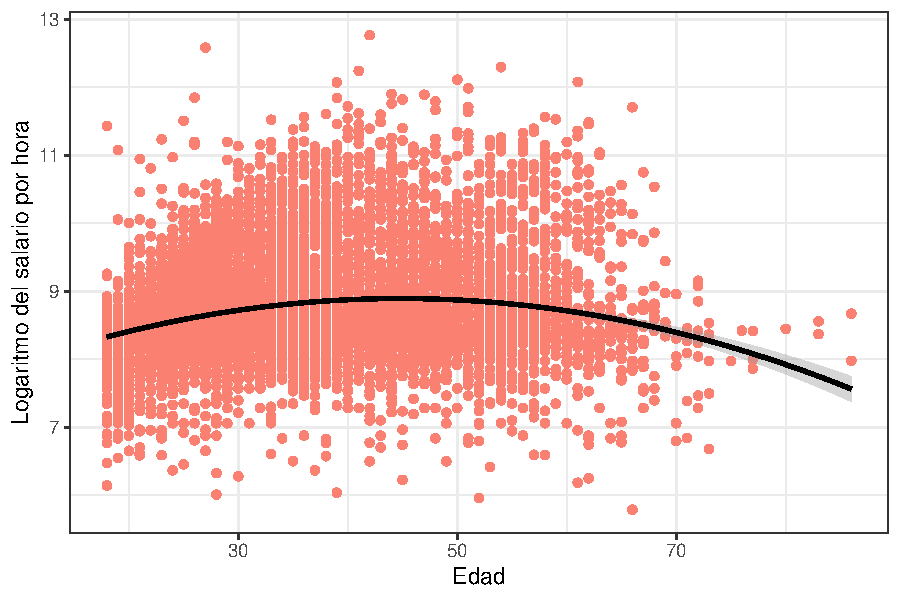
\includegraphics[width=0.7\textwidth]{imagenes/dispersion2.pdf}
             \label{fig:scatter2}
            \begin{minipage}{7\textwidth}
            \footnotesize
            \hspace{3cm} Fuente: Elaboración propia con GEIH 2024.
       
            \end{minipage}
        \end{figure}

\begin{table}[H]
    \centering
    \caption{Intervalos de confianza de la edad pico estimados por bootstrap}
    \begin{tabular}{cccccc}
        \hline
        \hline
        Confianza & Normal & Básico & Percentil & Bca \\
        \midrule
        95\% & $[43.7;45.91]$ & $[43.6;45.83]$ & $[43.82;46.04]$ & $[43.83;46.06]$ \\
        99\% & $[43.35;46.26]$ & $[43.19;46.12]$ & $[43.53;46.46]$ & $[43.53;46.48]$ \\
        \hline
        \hline 
    \end{tabular}\\
    \label{tab:intervalos_confianza}
    \footnotesize{Fuente: Elbaoración propia con GEIH, 2024.}
\end{table}

A partir de la gráfica y del peakage calculado se puede observar que el salario empieza a disminuir cuando una persona alcanza una edad de aproximadamente 45 años, estimación que según la tabla \ref{tab:intervalos_confianza} puede varias desde lo 43 años hasta lo 46 años en términos estadísticos. Ahora bien, es importante recalcar que utilizar intervalos de confianza construidos por Bootstrap para dicha edad pico estimado, es necesario debido a que no se puede confiar en la distribución del estimador de la edad pico. Este procedimiento nos permite estimar de forma acertada la varianza e intervalos de confianza del estimador de la edad pico calculando la varianza muestral debido a que el procedimiento de bootstrap realiza un remuestreó sin necesidad asumir una distribución. \\

Es crucial destacar la existencia de diversas metodologías de bootstrap, tales como el método normal, básico, de percentiles y Bca. Para este caso se decidió presentar las 4 metodologías debido a que se considera que las estimaciones del intervalo de confianza son robustas al tipo de bootstap utilizado.


\subsection{Brecha salarial por genero}
En segundo momento, se estimó una regresión simple del sexo contra el logaritmo del salario por hora para encontrar las brechas salariales entre hombres y mujeres en Bogotá, estos resultados se muestran a continuación:

\begin{table}[H]
\centering 
  \caption{Resultados regresión: logaritmo del salario vs Female} 
  \label{} 
  \resizebox{1\textwidth}{!}{
\begin{tabular}{@{\extracolsep{5pt}}lccc} 
\\[-1.8ex]\hline 
\hline \\[-1.8ex] 
 & \multicolumn{3}{c}{\textit{Variable dependiente:}} \\ 
\cline{2-4} 
\\[-1.8ex] & logaritmo del salario & \multicolumn{2}{c}{Logaritmo del salario} \\ 
\\[-1.8ex] & (1) & (2) & (3)\\ 
\hline \\[-1.8ex] 
 Mujer[1=Sí] & $-$0.04507$^{***}$ &  &  \\ 
  & (0.01460) &  &  \\ 
  & & & \\ 
  Mujer FWL [1=Sí]  &  & $-$0.09770$^{***}$ & $-$0.09770$^{***}$ \\ 
  &  & (0.01160) & (0.0123924) \\ 
  & & & \\ 
\hline \\[-1.8ex] 
Errores estándar & Convencionales & Convencionales & Bootstrap \\ 
Controles & No & Si & Si \\ 
Observaciones & 9,889 & 9,888 & 9,888 \\ 
R$^{2}$ & 0.00096 & 0.00713 & 0.00713 \\ 
R$^{2}$ ajustado & 0.00086 & 0.00702 & 0.00702 \\ 
Estadístico & 9.53032$^{***}$ (df = 1; 9887) & 70.94347$^{***}$ (df = 1; 9886) & 70.94347$^{***}$ (df = 1; 9886) \\ 
\hline 
\hline \\[-1.8ex] 
\textit{Nota:}  & \multicolumn{3}{r}{$^{*}$p$<$0.1; $^{**}$p$<$0.05; $^{***}$p$<$0.01} \\ 
\end{tabular} 
}
\end{table} 

Teniendo en cuenta la columna 1 de la tabla y que la variable Female toma el valor de 1 si la persona es mujer y 0 de lo contrario, se puede concluir que el hecho de ser mujer disminuye el salario de la persona por hora en promedio 4.5\% en comparación a los hombres. Es fundamental reconocer que esta estimación no abarca completamente la brecha salarial, ya que diversos factores como la educación, la experiencia, la profesión, entre otros, inciden tanto en el género como en el salario de una persona. Por lo tanto, omitir la consideración de estos elementos implica no capturar exclusivamente el impacto del género en la disparidad salarial entre hombres y mujeres, sino que sesga esta variable al verse influenciada por estos otros factores. A partir de este análisis se implementó un nuevo modelo incluyendo controles, ésta se muestra en la ecuación a continuación:

$$ln(w)=\beta_0+\beta_1 Female +\rho \Vec{X}+\varepsilon$$

Donde $\Vec{X}$ es un vector que incluye variables como: la edad, el nivel máximo de educación alcanzado, si la persona pertenece al sector formal, la profesión, las horas semanales trabajadas, si la persona tiene o no un segundo trabajo y el tamaño de la firma en la que trabaja. Este modelo fue implementado a partir del teorema de Frisch Waugh Lovell (FWL), el cual hace más eficiente la estimación dado un número alto de variables y de observaciones y se realiza a partir de los residuales de la variable explicativa sobre los residuales de la variable de interés. Además, se compara este resultado con la implementación de este mismo utilizando Bootstrap, que mediante remuestreo estima los errores estándar de los coeficientes corrigiendo por heteroscedasticidad y autocorrelación. En la columna 2 se observan los resultados de esta la primera estimación con FWL; a partir de estos se puede concluir que el hecho de ser mujer disminuye en promedio 9.77\% el salario por hora en comparación con un hombre. Este mismo resultado lo podemos observar en la columna 3, utilizando FWL con Bootstrap.  \\

Comparando los resultados obtenidos, se puede evidenciar que al momento de controlar por características similares “Equal Pay for Equal Work”, la brecha salarial por género persiste y se hace aún mayor por aproximadamente 5 puntos porcentuales. Adicionalmente se pasa de tener una capacidad predictiva baja (0.09\%) bajo la estimación sin controles a una capacidad predictiva mayor (0.7\%) utilizando controles. Por último, cuando se comparan los errores estándar de los modelos, se observa que el modelo inicial cuenta con un error estándar de 0.7, mientras que el modelo de FWL lo disminuye a 0.4 y se ve aún más disminuido cuando se utiliza Bootstrap (0.0125). Esto implica que el modelo que brinda mayor significancia estadística al resultado es el último, esto teniendo en cuenta la ecuación del estadístico t\footnote{$t=\frac{\hat{\beta}}{ee(\hat{\beta})}$} . \\

Con el propósito de entender en conjunto las relaciones que hemos analizado hasta ahora, se realizó una gráfica en la que se muestra la relación entre la edad y el logaritmo del salario por hora diferenciado por género. 

        \begin{figure}[H]
            \caption{Logaritmo del salario vs edad}
            \centering
            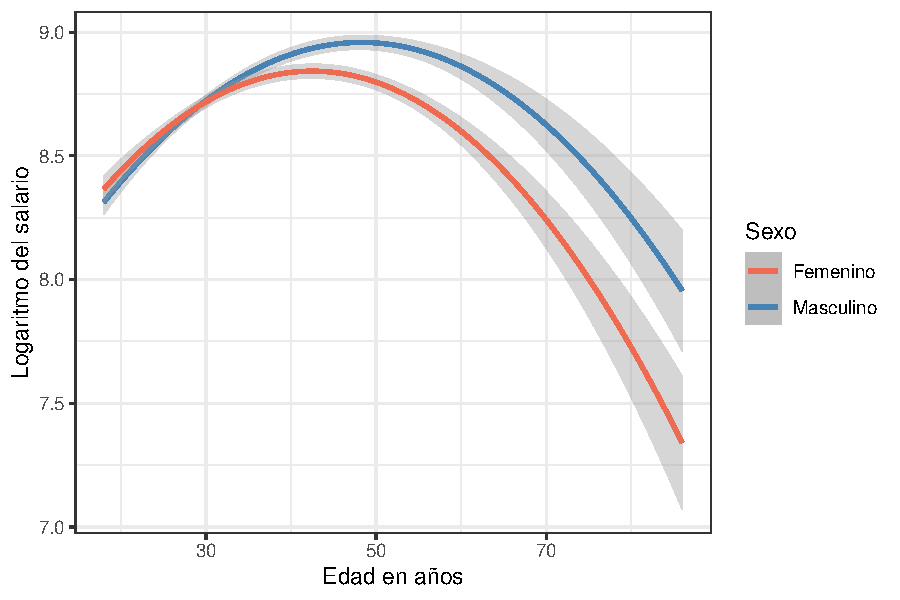
\includegraphics[width=0.8\textwidth]{imagenes/predict_by_zex.pdf}
             \label{fig:scatter1}
            \begin{minipage}{7\textwidth}
            \footnotesize
            \hspace{2cm} Fuente: Elaboración propia con GEIH 2024.
       
            \end{minipage}
        \end{figure}

A partir de esta, conjunto a los cálculos del peakage con Bootstrap se pueden resaltar varios aspectos. En primer lugar, se evidencia que existe una brecha salarial por género pero únicamente desde aproximadamente los 35 años de edad. Esto muestra entonces, que entre personas jóvenes los salarios entre hombres y mujeres son muy cercanos entre ellos, lo que implica que en la actualidad se está tratando de cerrar dicha brecha dándole oportunidades igualitarias a las personas jóvenes y así se cierre tanto a corto como a largo plazo dicha brecha de género. La brecha que persiste para personas mayores a aproximadamente los 35 años, muestra que en promedio los hombres tienen un mejor salario que las mujeres (lo que afirma los resultados obtenidos en la regresión. De la mano de esto, se calculó un peakage mayor para los hombres que para las mujeres (53 y 52 respectivamente), lo que significa que las mujeres alcanzan primero el cambio de efecto que tiene la edad sobre el salario. \\

\begin{table}[H]
    \centering
    \caption{Intervalos de Confianza de la edad pico para las mujeres estimados por bootstrap}
    \begin{tabular}{cccccc}
        \hline \hline
        Confianza & Normal & Básico & Percentil & Bca \\
        \midrule
        95\% & $[48.17;56.37]$ & $[47.56;55.71]$ & $[48.99;57.15]$ & $[49.17;57.69]$ \\
        99\% & $[46.88;57.66]$ & $[45.18;56.47]$ & $[48.23;59.52]$ & $[48.33;60.01]$ \\
        \hline
        \hline
    \end{tabular}
    \label{tab:intervalos_confianza_female}
    \begin{center}
    \footnotesize{\textbf{Fuente:} Elaboración propia con GEIH, 2024.}
\end{center}
\end{table}




\begin{table}[H]
    \centering
    \caption{Intervalos de Confianza de la edad pico para los hombres estimados por bootstrap}
    \begin{tabular}{cccccc}
        \hline \hline
        Confianza & Normal & Básico & Percentil & Bca \\
        \midrule
        95\% & $[49.52;56.47]$ & $[49.05;56.04]$ & $[50.17;57.16]$ & $[50.25;57.28]$ \\
        99\% & $[48.43;57.56]$ & $[47.00;56.75]$ & $[49.45;59.21]$ & $[49.5;50.34]$ \\
        \hline
        \hline
    \end{tabular}
    \label{tab:intervalos_confianza_male}
    \begin{center}
    \footnotesize{\textbf{Fuente:} Elaboración propia con GEIH, 2024.}
\end{center}
\end{table}


 Sin embargo, al observar los intervalos de confianza construidos por Bootstrap, los cuales se encuentran en la siguiente tabla, se observa que, los hombres y mujeres comparten gran parte de su rango (a excepción de 1 a 2 puntos porcentuales), esto puede explicar la proximidad de sus peakages, implicando que no existe una brecha significativa de edad de punto máximo, aunque persista una de los salarios.


\section{Analisis predictivo}

\begin{table}[H] \centering 
  \caption{} 
  \label{} 
\begin{tabular}{@{\extracolsep{5pt}} ccc} 
\\[-1.8ex]\hline 
\hline \\[-1.8ex] 
 & MODELO & MSE Muestral. \\ 
\hline \\[-1.8ex] 
 & Modelo 1 & 0.714316354386539 \\ 
 & Modelo 2 & 0.492045722021568 \\ 
 & Modelo 3 & 0.713659312388961 \\ 
 & Modelo 4 & 22.2570614869402 \\ 
 & Modelo 5 & 0.266853718759632 \\ 
 & Modelo 6 & 0.261430634465058 \\ 
 & Modelo 7 & 0.277722312155594 \\ 
\hline \hline
\end{tabular} 

\begin{center}
    \footnotesize{Fuente: Elaboración propia con GEIH, 2024.}
\end{center}
\end{table} 


En la tabla previa se muestran los errores de predicción medios de los 7 modelos lineales propuestos utilizando 70\% de la muestra para entrenamiento y el restante 30\% para el cálculo de estos errores. Los primeros 2 modelos se refieren a los propuestos por el enunciado y analizados en el documento, los 3 y 4 exploran otros tipos de complejidad lineal, donde el tercero modela el logaritmo del salario según ocho polinomios de la edad y el cuarto modela interacciones polinomiales con las variables de control utilizadas para el segundo modelo. En general, estos primeros cuatro modelos tienen una alta incidencia de errores de predicción fuera de muestra, ya que sus MSE’s se encuentran (al rededor) por encima del 50\%, especialmente el cuarto modelo, el cual tiene un MSE extremadamente alto y es un claro ejemplo de sobre ajuste. En el reporte, estos cuatro modelos se entrenaron sobre la base de datos que se ha utilizado, y en los tres restantes se realizó un procesamiento de datos adicional. \\

Este procesamiento de datos para predicción resulta sustancialmente diferente al utilizado para econometría explicativa. En este sentido, se utilizó la base de datos completa y se filtraron las variables que tuvieran menos de 20\% de observaciones faltantes y se eliminaron algunas observaciones clasificadas en clases muy poco comunes. Después de esta primera selección se clasificaron las variables escogidas en tipos de variables (continuas, ordinales, categóricas y binarias) y se modificaron según su clase. Las variables continuas y ordinales se normalizaron para controlar por la escala de medición (a excepción del logaritmo del salario), las categóricas se dummyficaron excluyendo una categoría para evitar multicolinealidad perfecta y se corrigieron las dummys codificadas en 1-2 para que quedaran en 1-0.  \\

Posteriormente se construyó la matriz de correlación de la base completa y se eligió una sola variable de los conjuntos con correlación absoluta mayor a .999, primando las variables continuas sobre todas las demás debido a la naturaleza de nuestra variable de interés (también continua) y para evitar incluir variables que puedan sobreajustar nuestros modelos. Finalmente se utilizó la metodología de k-vecinos cercanos (kNN por sus siglas en inglés), con k = 10, para imputar los valores faltantes de las variables seleccionadas en los pasos anteriores. La normalización de las variables es necesaria también para el uso del kNN. \\

Utilizando esta base de datos alternativa se construyeron los modelos 5, 6 y 7. Para el quinto y el sexto modelo se propuso una forma funcional extensa, en la cual las variables continuas están sumadas hasta su polinomio de grado dos, y las demás variables adicionan, sin interacciones. Basándose en este modelo se utilizó el algoritmo de forward selection para definir la forma funcional del modelo 5 y backward selection para definir la del sexto modelo. El séptimo modelo es la intersección de las variables elegidas por ambos algoritmos.
Como se evidencia en la tabla de los errores de predicción, estos últimos tres modelos presentan una capacidad predictiva significativamente mayor a la de los modelos previamente discutidos, rondando el error medio de .26. El modelo con menor error cuadrático medio fuera de muestra fue el seleccionado mediante backward selection donde se eligieron treinta y tres variables independientes.


$$ln(w)= X\beta+U$$ 

Aunque el modelo es relativamente superior al resto, este también En el APENDICE se encuentra la especificación del modelo. Este modela el logaritmo del salario por hora como una combinación de 33 variables individuales, con algunas de ellas al cuadrado. Entre las variables que incrementan la predicción del salario se encuentran el sexo (masculino), el nivel educativo más alto alcanzado, el grado escolar aprobado, el tamaño de la firma, la antigüedad de empleo en la firma (de manera cuadrática), el valor del subsidio familiar, si le hicieron la entrevista en diciembre, transferencias por pagos alimenticios/divorcio (de manera cuadrática). Las variables que reducen la predicción de salario son: oficio, recibir transferencias de otros hogares, haber cursado educación terciaria, horas totales trabajadas, si dedico mayor tiempo de su semana pasada a los oficios del hogar, si no cotiza pensión o es pensionado, el valor del subsidio de transporte, el valor estimado de pago en especia (vivienda) (de manera cuadrática), el valor estimado de pago en especia (transporte), el valor estimado de otros pagos en especial, pagos por pensiones/jubilaciones (de manera cuadrática), el valor recibido de instituciones nacionales/extranjeras e ingresos por ayudas de hogares. Finalmente hay algunas variables que afectan la predicción del salario de manera cuadrática. El ingreso total observado, el valor de la última bonificación anual, el valor del subsidio educativo y del subsidio de alimentación, aumentan el salario de manera marginalmente decreciente. Por su parte, rentas no laborales del mes anterior y el ingreso total reducen de manera marginalmente decreciente la predicción del salario. \\



En el ANEXO se encuentra la especificación del modelo. Este modela el logaritmo del salario por hora como una combinación de 33 variables individuales, con algunas de ellas al cuadrado. Entre las variables que incrementan la predicción del salario se encuentran el sexo (masculino), el nivel educativo más alto alcanzado, el grado escolar aprobado, el tamaño de la firma, la antigüedad de empleo en la firma (de manera cuadrática), el valor del subsidio familiar, si le hicieron la entrevista en diciembre, transferencias por pagos alimenticios/divorcio (de manera cuadrática). Las variables que reducen la predicción de salario son: oficio, recibir transferencias de otros hogares, haber cursado educación terciaria, horas totales trabajadas, si dedico mayor tiempo de su semana pasada a los oficios del hogar, si no cotiza pensión o es pensionado, el valor del subsidio de transporte, el valor estimado de pago en especia (vivienda) (de manera cuadrática), el valor estimado de pago en especia (transporte), el valor estimado de otros pagos en especial, pagos por pensiones/jubilaciones (de manera cuadrática), el valor recibido de instituciones nacionales/extranjeras e ingresos por ayudas de hogares. Finalmente hay algunas variables que afectan la predicción del salario de manera cuadrática. El ingreso total observado, el valor de la última bonificación anual, el valor del subsidio educativo y del subsidio de alimentación, aumentan el salario de manera marginalmente decreciente. Por su parte, rentas no laborales del mes anterior y el ingreso total reducen de manera marginalmente decreciente la predicción del salario. \\

        \begin{figure}[H]
            \caption{Distribución del MSE estimado}
            \centering
            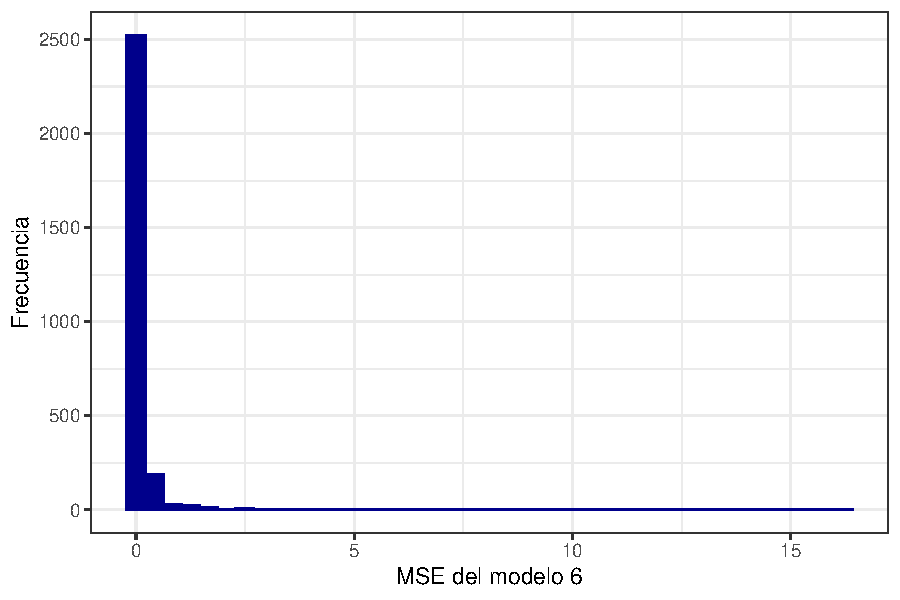
\includegraphics[width=0.8\textwidth]{imagenes/histograma_mse.pdf}
             \label{fig:hist_mse}
            \begin{minipage}{7\textwidth}
            \footnotesize
            \hspace{2cm} Fuente: Elaboración propia con GEIH 2024.
            \end{minipage}
        \end{figure}

Aunque el modelo es relativamente superior al resto, este también presenta problemas de predicción para algunas observaciones de la base de testeo. Con el fin de comprender mejor la naturaleza de estos errores se calculó la distribución de los errores cuadráticos para la base de prueba la cual se observa en la figura \ref{fig:hist_mse} y partir de ella se extrajeron las observaciones con MSE’s mayores a tres veces la desviación estándar del mismo MSE. De las 23 observaciones que cumplen con este criterio únicamente 5 son producto de sub-estimaciones del modelo, lo cual indica que para las observaciones de las colas de la distribución el modelo propuesto tiende a sobre-estimar el salario. En este sentido, las observaciones atípicas (MSE mayor a tres veces la desviación del MSE) al ser sobreestimaciones no implicarían un problema para la DIAN y no requerirían de una investigación especifica. De todos modos, la gran mayoría de errores de predicción tienen una distancia cuadrática menor a 1,72 (tres veces la desviación estándar del MSE), lo cual indica que el modelo se aproxima satisfactoriamente a la gran mayoría de observaciones \\

\begin{table}[h]
    \centering
    \caption{Resultado de LOOCV}
    \begin{tabular}{lccc}
        \hline
        \textbf{Estimación} & \textbf{Promedio}  \textbf{MSE}  \textbf{LOOCV} \\
        \hline
        Backward (modelo 6) & 0.2727 \\
        Forward (modelo 7) & 0.2705 \\
        \hline
    \end{tabular}
    \label{tab:estimaciones loocv}
    \begin{center}
        \footnotesize{Fuente: Elaboración propia con GEIH, 2024.}
    \end{center}
\end{table}



Para los modelos 5 y 6 se estimaron los MSE medios mediante la metodología LOOCV para corroborar las estimaciones hechas dividiendo la base de datos en entrenamiento y testeo. Como se evidencia en la tabla previa, las estimaciones por LOOCV muestran valores más pequeños de error, y debido a que este método de estimación es más preciso, nuestros modelos son mejores de lo que se había estimado previamente. La precisión del LOOCV se basa en su capacidad de minimizar la incidencia de la aleatoriedad en la particion test-train, al calcular la media de los errores excluyendo una observación a la vez. En este sentido, si observaciones influyentes o atípicas se concentran en el set de prueba, puede que la metodología de testeo sobre el 30\% sobre estime el MSE medio fuera de muestra, mientras que el LOOCV promedia los errores sobre cada observación y por lo tanto esta concentración no incide en la estimación.

\newpage
\section*{Referencias}

\begin{itemize}
    \item[$\bullet$] DIAN. (2022). Informe 2022: Rendición de Cuentas Prospectiva 2023-2026. \\https://www.dian.gov.co/dian/entidad/Documents/Informe-2022- Rendicion-de-Cuentas-Prospectiva-2023-2026.pdf

\end{itemize}

\newpage
\section*{Anexos}

\begin{table}[H] \centering 
  \caption{Resultados del modelo 6} 
  \label{} 
  \resizebox{0.25\textwidth}{!}{
\begin{tabular}{@{\extracolsep{5pt}}lc} 
\\[-1.8ex]\hline 
\hline \\[-1.8ex] 
 & \multicolumn{1}{c}{\textit{Variable dependiente:}} \\ 
\cline{2-2} 
\\[-1.8ex] & Logaritmo del salario \\ 
\hline \\[-1.8ex] 
 sex & 0.057$^{***}$ \\ 
  & (0.007) \\ 
  & \\ 
 p6210 & 0.050$^{***}$ \\ 
  & (0.004) \\ 
  & \\ 
 p6210s1 & 0.035$^{***}$ \\ 
  & (0.006) \\ 
  & \\ 
 oficio & $-$0.029$^{***}$ \\ 
  & (0.004) \\ 
  & \\ 
 p7505 & $-$0.042$^{***}$ \\ 
  & (0.007) \\ 
  & \\ 
 college & $-$0.129$^{***}$ \\ 
  & (0.014) \\ 
  & \\ 
 totalHoursWorked & $-$0.177$^{***}$ \\ 
  & (0.003) \\ 
  & \\ 
 sizeFirm & 0.050$^{***}$ \\ 
  & (0.004) \\ 
  & \\ 
 p6240\_4 & $-$0.132$^{***}$ \\ 
  & (0.020) \\ 
  & \\ 
 p6920\_2 & $-$0.198$^{***}$ \\ 
  & (0.011) \\ 
  & \\ 
 I(p6426$\hat{\mkern6mu}$2) & 0.004$^{***}$ \\ 
  & (0.001) \\ 
  & \\ 
 p6585s1a1 & 0.003 \\ 
  & (0.005) \\ 
  & \\ 
 I(p6585s1a1$\hat{\mkern6mu}$2) & $-$0.001$^{**}$ \\ 
  & (0.0003) \\ 
  & \\ 
 p6585s2a1 & $-$0.013$^{***}$ \\ 
  & (0.003) \\ 
  & \\ 
 p6585s3a1 & 0.014$^{***}$ \\ 
  & (0.003) \\ 
  & \\ 
 p6585s4a1 & 0.011 \\ 
  & (0.010) \\ 
  & \\ 
 I(p6585s4a1$\hat{\mkern6mu}$2) & $-$0.0001 \\ 
  & (0.0002) \\ 
  & \\ 
 I(p6600s1$\hat{\mkern6mu}$2) & $-$0.0001$^{***}$ \\ 
  & (0.00005) \\ 
  & \\ 
 p6610s1 & $-$0.011$^{***}$ \\ 
  & (0.003) \\ 
  & \\ 
 p6620s1 & $-$0.013$^{**}$ \\ 
  & (0.005) \\ 
  & \\ 
 p6630s6a1 & 0.015$^{**}$ \\ 
  & (0.007) \\ 
  & \\ 
 I(p6630s6a1$\hat{\mkern6mu}$2) & $-$0.0004$^{**}$ \\ 
  & (0.0002) \\ 
  & \\ 
 p7500s1a1 & $-$0.089$^{***}$ \\ 
  & (0.005) \\ 
  & \\ 
 I(p7500s1a1$\hat{\mkern6mu}$2) & 0.002$^{***}$ \\ 
  & (0.0002) \\ 
  & \\ 
 I(p7500s2a1$\hat{\mkern6mu}$2) & $-$0.001$^{***}$ \\ 
  & (0.0001) \\ 
  & \\ 
 I(p7500s3a1$\hat{\mkern6mu}$2) & 0.0002 \\ 
  & (0.0003) \\ 
  & \\ 
 p7510s3a1 & $-$0.00003 \\ 
  & (0.003) \\ 
  & \\ 
 I(ingtotob$\hat{\mkern6mu}$2) & $-$0.061$^{***}$ \\ 
  & (0.005) \\ 
  & \\ 
 ingtot & $-$0.012 \\ 
  & (0.046) \\ 
  & \\ 
 I(ingtot$\hat{\mkern6mu}$2) & 0.005 \\ 
  & (0.005) \\ 
  & \\ 
 mes\_12 & 0.001 \\ 
  & (0.012) \\ 
  & \\ 
 p6920\_3 & $-$0.276$^{***}$ \\ 
  & (0.032) \\ 
  & \\ 
 iof3h & $-$0.031$^{***}$ \\ 
  & (0.004) \\ 
  & \\ 
 ingtotob & 0.862$^{***}$ \\ 
  & (0.047) \\ 
  & \\ 
 Constant & 8.894$^{***}$ \\ 
  & (0.007) \\ 
  & \\ 
\hline \\[-1.8ex] 
Observaciones & 6,515 \\ 
R$^{2}$ & 0.877 \\ 
R$^{2}$ Ajustado & 0.876 \\ 
Residual Estd. Error & 0.250 (df = 6480) \\ 
Estadistico F & 1,357.429$^{***}$ (df = 34; 6480) \\ 
\hline 
\hline \\[-1.8ex] 
\textit{Note:}  & \multicolumn{1}{r}{$^{*}$p$<$0.1; $^{**}$p$<$0.05; $^{***}$p$<$0.01} \\ 
\end{tabular} 
}
\end{table}

\end{document}